\chapter{Introduction}

\section{Introduction to Microscopy}
\label{sec:microscopy}

The principle of optical magnification was known at least as early 
as the 1st Century CE. The enhancement of resolving power for 
objects viewed through spherical glass objects filled with water 
(a kind of pro-lens) was noted by Seneca and some of his 
contemporaries\cite{seneca1971naturales}. Even after the collapse 
of the Roman Empire and Europe entered the Dark Ages other scholars, 
such as Ibn al-Haytham, noted and investigated the phenomenon of 
optical magnification through convex-planar pieces of 
glass\cite{nasr1968science}. It is an amusing anecdote, especially 
given the importance which microscopy has come to furthering 
biological understanding, that it was not until the end of 13th 
Century  when Roger Bacon penned his \textit{Opus majus} that a 
practical use for magnification could be found - eyeglasses. It 
was a further 300 years until the first telescopes and microscopes 
were developed. The exact date and inventor of the first telescope 
is unknown, but the credit is usually attributed to one of four 
Dutchmen at the start of the 17th Century; Hans Janssen, his son 
Zacharias, Hans Lippershey, or Jacob Metius. Likewise, precise date 
and inventor of the first microscope is not known, but the invention 
did occur at around the same time and the term was coined by Giovanni 
Faber in 1625\cite{bardell2004invention}. It is interesting to note 
that the invention of microscopes and telescopes are so closely linked, 
especially in light of the origin of adaptive optics technology which 
we will address shortly. The true power microscopes to yield novel 
biological understanding was first popularised by Robert Hooke and then
later by Antonie van 
Leeuwenhoek\cite{hooke1665micrographia, chung2017pioneers}. Since then, 
the microscope has been and remains one of the premiere tools enabling 
biological discoveries.

\subsection{Fluorescence microscopy}
\label{subsec:fluorescence}

Microscopes allowed biologists to visualise structures well below the 
length-scale available to the naked eye. However, living material still 
remained resistant to optical examination due to a number of properties: 
strong scattering properties, particularly for wavelengths of light 
within the visible spectrum; transparency; innate light-protective 
mechanisms to prevent damage from solar radiation. Phase contrast 
microscopy could solve some of the issues when visualising otherwise 
transparent samples\cite{burch1942phase}. More typically microscopy 
samples were chemically fixed as these samples were more stable and 
easier to refractive index match to the microscope. Histological staining 
was, for decades, the primary method for revealing biological structures\cite{alturkistani2016histological}. The properties and function 
of living material were then inferred from fixed samples. This was, as one 
author put it, ``like reconstructing a football game from a series of still 
pictures,...an arduous (and some would say hopeless) 
endeavour''\cite{yuste2005fluorescence}. 

Fluorescence is the property of atoms and molecules whereby they emit light
after stimulation from an external energy source. In steady-state conditions 
(i.e. without an external energy source) the electrons of the atom or 
molecule are found in the ground state. Photons from the external energy 
source are absorbed by these electrons, raising them to excited single states.
When these excited electrons return to the ground state, they can release 
their energy as a photon - it is this phenomenon which is called fluorescence\cite{ghiran2011introduction}. For atoms, these energy states are
reasonably discrete and (for the lowest levels) easy enough to draw in 
Jab\l{}onski diagrams. Molecules capable of fluorescence, called fluorophores, 
have broad ``energy bands'' of possible excitation and emission wavelengths. 
Additionally, the absorption and emission cross-sections are not the same for
all wavelengths. This leads to excitation and emission spectra for fluorescent
molecules. Figure~\ref{fig:GFP_emission_absorption_spectra} shows the 
excitation and emission spectra for Green Fluorescent Protein (GFP), generated 
with SpekCheck\cite{phillips2018spekcheck}.

\begin{figure}[h]
	\centering
	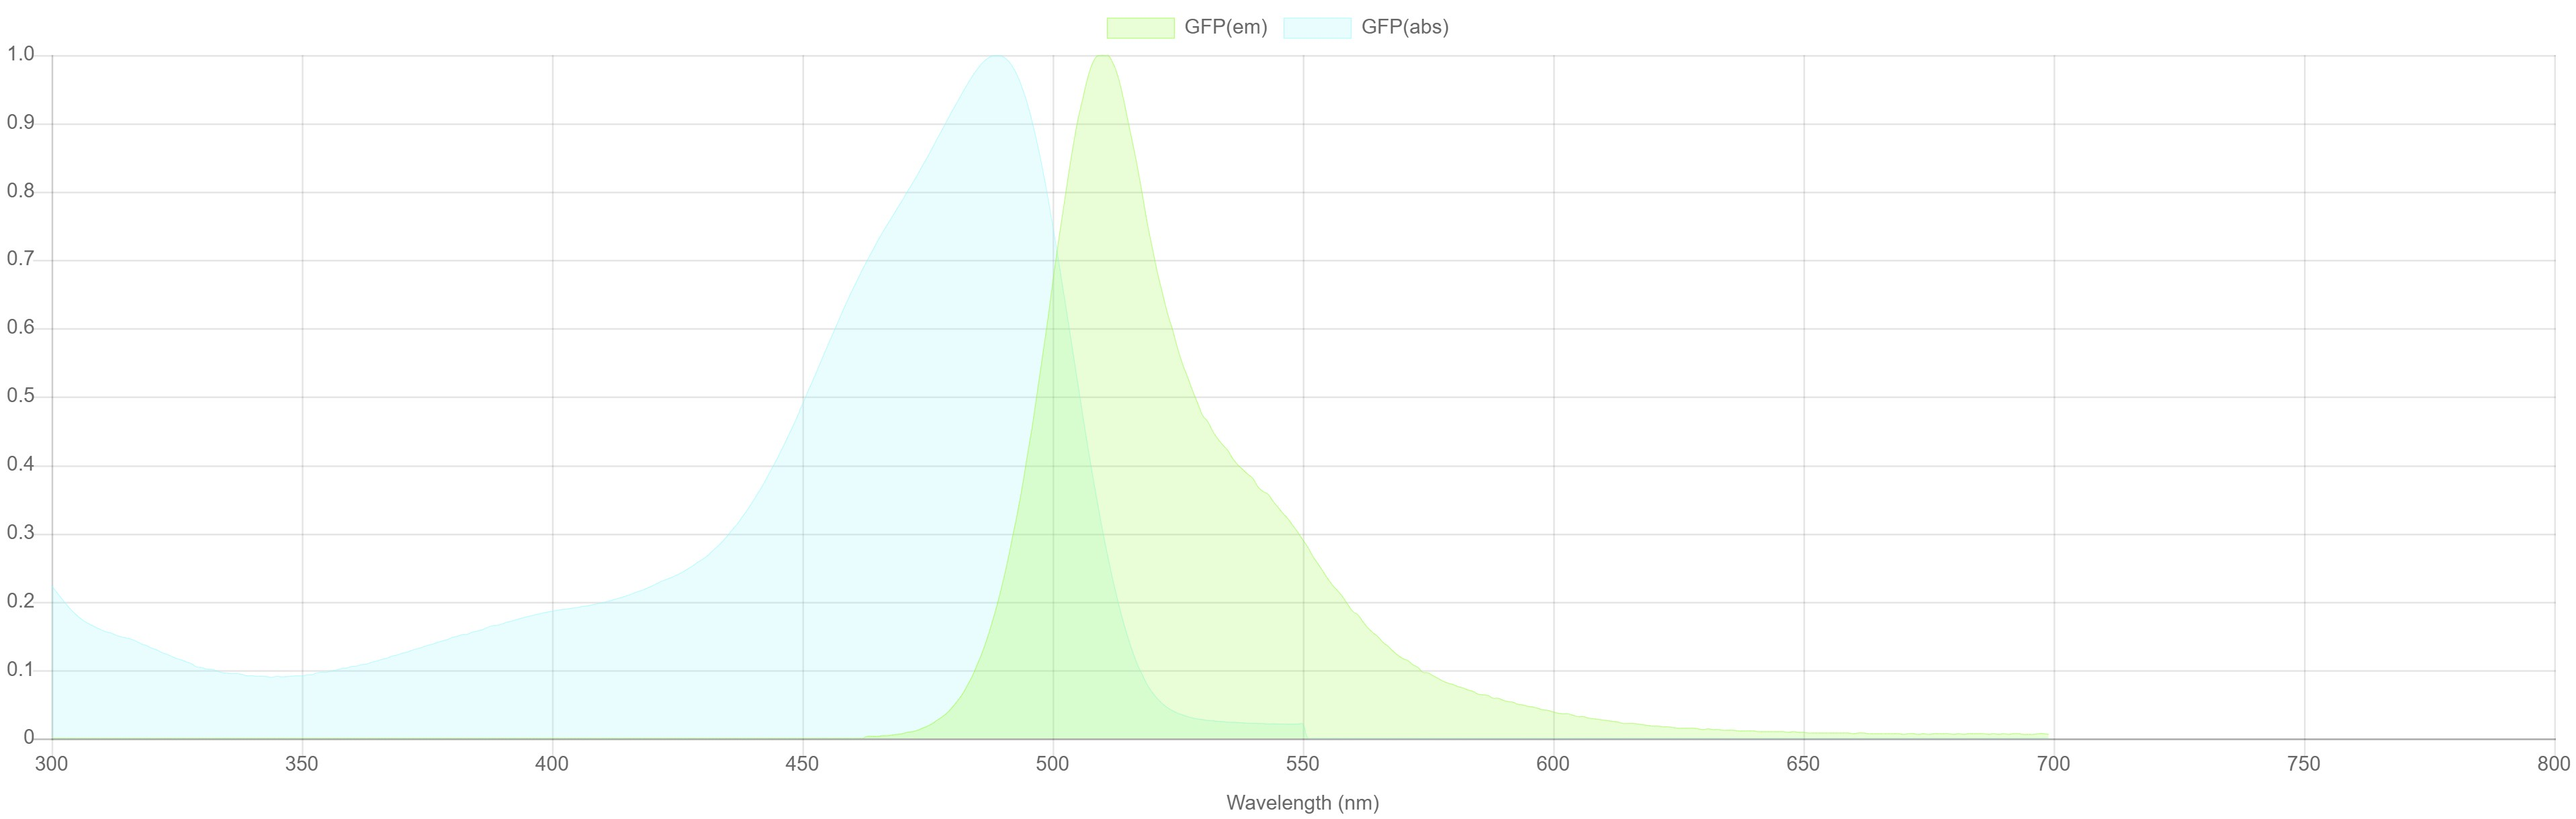
\includegraphics[width=\textwidth]{images/GFP_emission_absorption_spectra.jpg}
	\caption{Example excitation (blue) and emission (green) spectra for Green Fluorescent Protein. Generated with SpekCheck\cite{phillips2018spekcheck}}
	\label{fig:GFP_emission_absorption_spectra}
\end{figure}

The first fluorescence microscopes were developed at the beginning of the 20th Century\cite{renz2013fluorescence,yuste2005fluorescence}. The real power of 
fluorescence microscopy came as the specificity of labelling improved. The 
first iteration of this was the development of antibody fluorescent labelling 
which allowed for, among other things, localisation of viral particles in 
biological 
cultures\cite{coons1942demonstration,coons1951fluorescent,weller1954fluorescent}.
The second, and arguably more profound, iteration was the discovery and 
cloning of \textit{Aequorea victoria} GFP, and the development of chromatic
variants\cite{prasher1992primary,heim1996engineering}. This allowed for 
specific proteins of interest to be individually labelled and for biologists 
to monitor gene-expression\cite{chalfie1994green}. Since then, additional 
properties of fluorescent proteins, such as their conformational changes 
in response to binding events, environmental changes or enzymatic activity, 
have been utilised to great effect\cite{toseland2013fluorescent}. 
Fluorescence microscopy has allowed biologists to visualise dynamic biological
processes in real time.

\subsection{Resolution}
\label{subsec:resolution}

A fundamental property of all microscopes and microscopy images is that of 
resolution - the minimum separation between two objects where they can still
be determined to be two distinct objects. Consider an optical plane, 
$\textbf{O}$, where a biological specimen is placed - the `sample plane'. Also
consider a separate optical plane, $\textbf{O'}$, where the image of the
specimen is formed - the `image plane'. The microscope, with circular entrance
and exit pupils, maps the field distributions between $\textbf{O}$ and 
$\textbf{O'}$. Figure~\ref{fig:simplified_microscope_layout} shows a schematic
of this simplified system.

\begin{figure}[h]
	\centering
	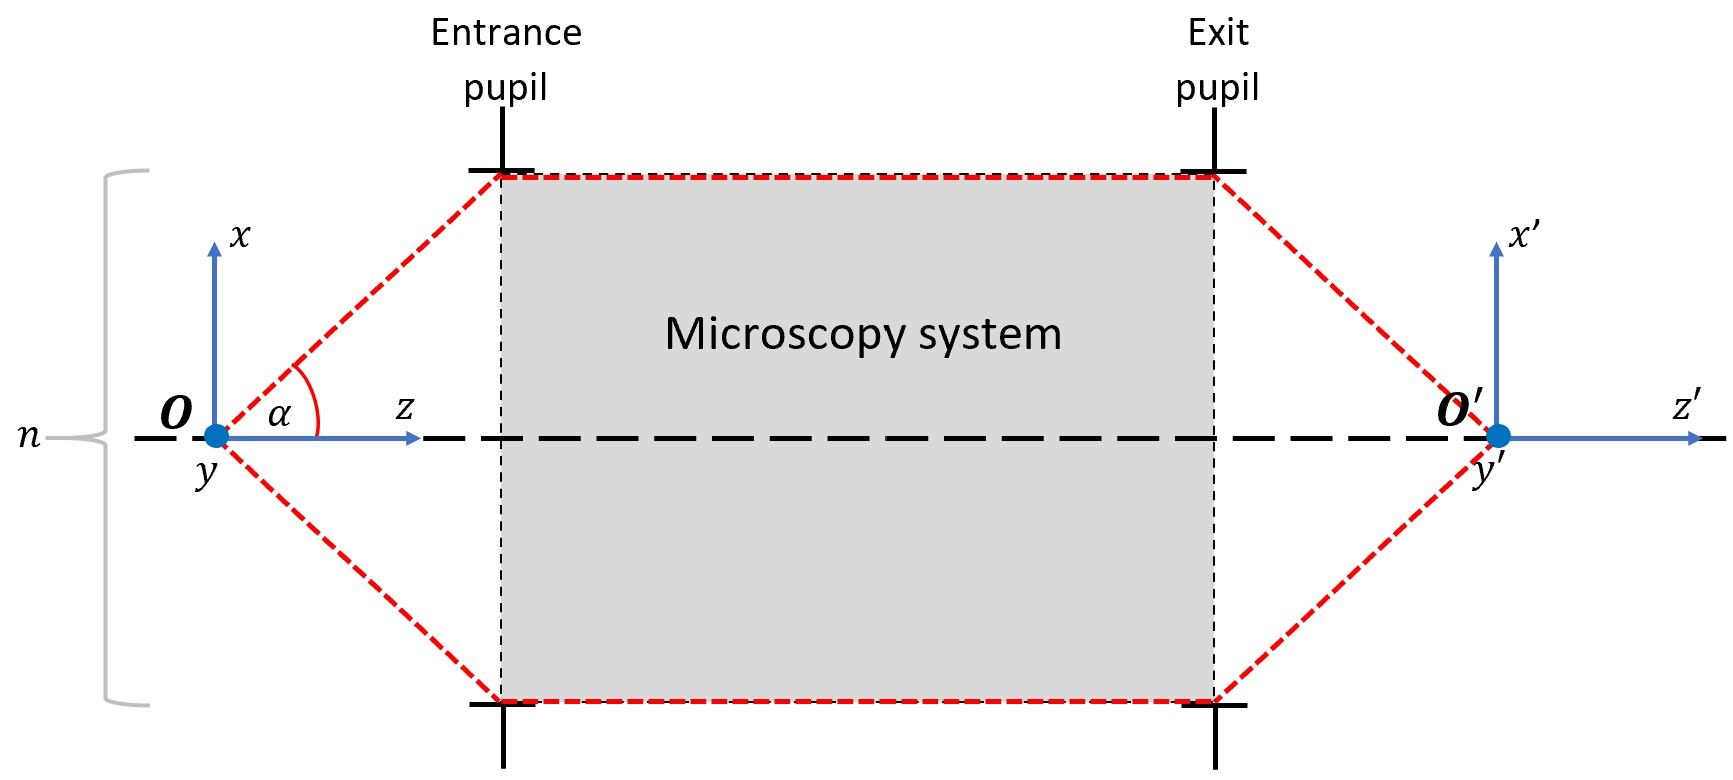
\includegraphics[width=\textwidth]{images/simplified_microscope_layout.jpg}
	\caption{A simplified schematic of a light microscopy imaging system. A specimen 
		is placed at the sample plane, $\textbf{O}$, in refractive index, $n$. Light 
		rays emerging from $\textbf{O}$ are collected by the entrance pupil. These 
		rays process through the microscope system before emerging at the exit pupil 
		and being focused at the image plane, $\textbf{O'}$. The light rays which 
		form and angle with the optical axis, $\textbf{OO'}$, of $\alpha$ are called
		marginal rays. Marginal rays are the highest diffraction order collectable by
		the entrance pupil and therefore the microscope system as a whole.}
	\label{fig:simplified_microscope_layout}
\end{figure}

Consider a point source located at $\textbf{O}$ isotopically emitting 
monochromatic light of wavelength $\lambda$. Every ray forms an angle, 
$\theta$, with the optical axis $\textbf{OO'}$. The highest angle collected
by the entrance pupil is $\alpha$. A point source can be considered an 
infinitely fine diffraction grating and $\alpha$ determines the highest 
diffraction order which the entrance pupil - i.e. the microscope
objective aperture - can collect\cite{davidson2002optical}. Considering this 
and, more generally, the diffraction of light through a circular aperture 
it is possible to obtain that the field intensity at \textbf{O'}, $I(v)$, is 
proportional to\cite{goodman2005introduction,born2013principles,antonello2014optimisation}:

\begin{equation}\label{eq:image_field_insentity}
I(v) \propto \left|\frac{2J_{1}(v)}{v}\right|^2,
\end{equation}

where $J_{1}(v))$ is the first-order Bessel function of the first kind of
the variable $v$\cite{watson1995treatise}. $v$ is the normalised lateral 
co-ordinate given by\cite{wilson1984theory}:

\begin{equation}\label{eq:normalised_lateral}
v = \frac{2\pi}{\lambda}rn\sin(\alpha).
\end{equation}

$r$ is the radial displacement in the image plane $\textbf{O'}$, $r = \sqrt{x'^{2} + y'^{2}}$. 
A useful quantity, and one often cited by microscope objective manufacturers, 
is the numerical aperture, $NA = n\sin(\alpha)$. The Rayleigh criterion 
determines that the limit at which two point objects can be meaningfully 
separated is when the central maxima of one diffraction pattern lies in the
first minimal of the other\cite{rayleigh1874xii,rayleigh1880investigations}. For a first order Bessel 
function, this occurs at $v \approx 1.22\pi$. Therefore the lateral resolution 
limit, $r_l$ is often quoted as:

\begin{equation}\label{eq:lateral_res}
r_l \approx \frac{1.22\lambda}{2NA}
\end{equation}

otherwise known as the Abbe diffraction limit\cite{abbe1873beitrage}. Through
a similar process and considering the field intensity along the $z'$ axis, the
axial resolution, $r_a$, is given as\cite{pawley2006handbook}:

\begin{equation}\label{eq:axial_res}
	r_a \approx \frac{2\lambda n}{NA^{2}}
\end{equation}

Figure~\ref{fig:Airy_ring_2_object_seperation} shows two 
diffraction-limited point objects at variable lateral separations. For 
lateral separations less than $r_{l}$ the field intensities resemble a single 
point source in the image plane. For lateral seperations at or above $r_{l}$ 
the intensity contributions from the two objects are distinguishable as 
separate.

\begin{figure}[h]
	\centering
	\begin{subfigure}{0.49\textwidth}
		\centering
		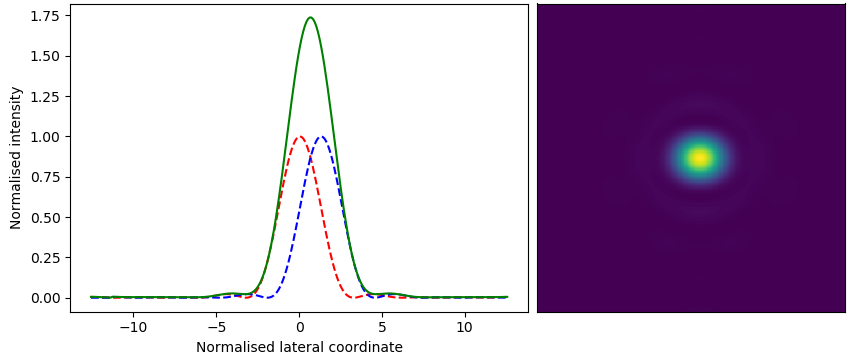
\includegraphics[width=\linewidth]{images/Airy_ring_2_object_seperation_0_5.png}
		\caption{Object separation = $0.41\text{r}_{\text{l}}$}
		\label{fig:Airy_ring_2_object_seperation_0_5}
	\end{subfigure}
	\begin{subfigure}{0.49\textwidth}
		\centering
		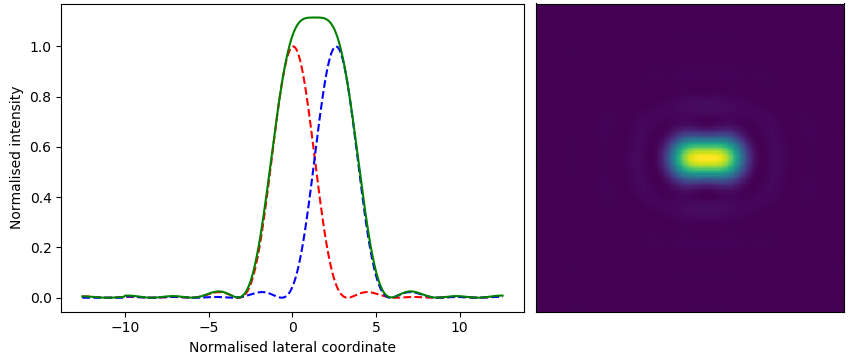
\includegraphics[width=\linewidth]{images/Airy_ring_2_object_seperation_1_0.png}
		\caption{Object separation = $0.82\text{r}_{\text{l}}$}
		\label{fig:Airy_ring_2_object_seperation_1_0}
	\end{subfigure}
	\begin{subfigure}{0.49\textwidth}
		\centering
		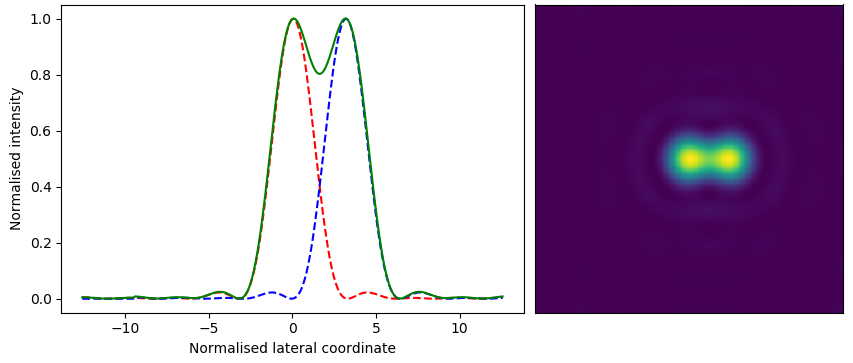
\includegraphics[width=\linewidth]{images/Airy_ring_2_object_seperation_1_22.png}
		\caption{Object separation = $1.0\text{r}_{\text{l}}$}
		\label{fig:Airy_ring_2_object_seperation_1_22}
	\end{subfigure}
	\begin{subfigure}{0.49\textwidth}
		\centering
		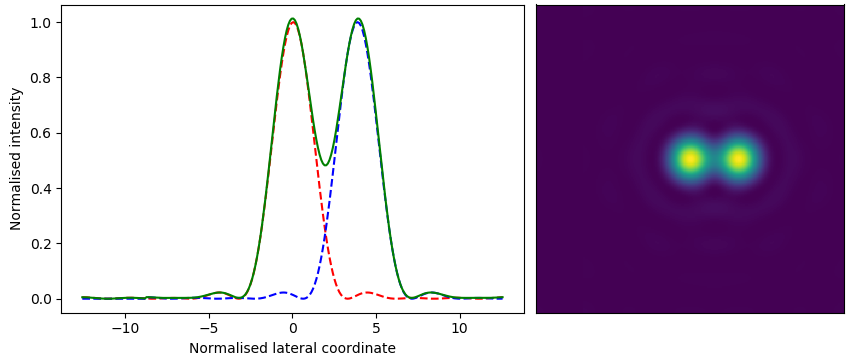
\includegraphics[width=\linewidth]{images/Airy_ring_2_object_seperation_1_5.png}
		\caption{Object separation = $1.23\text{r}_{\text{l}}$}
		\label{fig:Airy_ring_2_object_seperation_1_5}
	\end{subfigure}
	\caption{Illustration of the resolution limit as determined by the Rayleigh 
		criterion. Each subfigure shows a line profile and 2D plot of the field 
		intensity distributions of both of the two diffraction limited point 
		objects. For two point objects separated by $< r_{l}$, \textbf{(a)} \& 
		\textbf{(b)}, they are not separable as individual objects. At a 
		separation $\ge r_{l}$, \textbf{(c)} \& \textbf{(d)}, the two point 
		objects are separable.}
	\label{fig:Airy_ring_2_object_seperation}
\end{figure}

Several approximations had to be made to obtain Equations~\ref{eq:lateral_res}
and~\ref{eq:axial_res}. Firstly, the Fraunhofer and paraxial approximations are
assumed to hold\cite{goodman2005introduction}. Obviously the microscope system
has been greatly simplified to essentially just the entrance and exit pupils. 
More complex but accurate models for modern microscopy set-ups have been 
demonstrated\cite{torok2007optical, foreman2011computational}. Finally, this
idealised system only considers the shape of the apertures - i.e. the entrance
and exit pupils - and the wavelength of light. If one were to observe objects 
such as these, with these field distributions corresponding to well-specified
models, there would be no resolution limit at all\cite{den1997resolution}. In 
practice, the field distributions of objects are not precisely known, therefore
determining the location of the first minima is not as simple as it has been 
presented here. The first minima may not even be radially symmetric. 

Furthermore, the `true' resolution achievable by a microscopy system is affected 
by other factors such as the signal-to-noise ratio of an image, coherence 
conditions of illumination, apodization, descretisation errors for digital 
cameras, the to name a few\cite{den1997resolution}. There have been attempts to 
develop alternative resolution measurements for point objects\cite{ram2006beyond}. 
Unfortunately, the actual resolution acheived in biological samples varies 
across the image plane, determined by factors such as the labelling density of 
the underlying biological specimen\cite{culley2017nanoj}. The `true' resolution 
of a system for a given sample is therefore a quantity which is impossible to 
determine analytically. The ideal lateral and axial resolutions in 
Equations~\ref{eq:lateral_res} and~\ref{eq:axial_res} are nonetheless useful
quantities as the theoretical, ideal resolution limit of a microscopy system.

\section{Super-resolution Microscopy}
\label{sec:super_res}

\begin{itemize}
	\item Introduction to the fact that there are methods for overcoming the resolution limit and different techniques with different pros/cons
\end{itemize}

\subsection{Structured Illumination Microscopy}
\label{subsec:SIM}

\begin{itemize}
	\item General overview of SIM, particularly Gustafsson-style SIM.
\end{itemize}

\section{Optical Aberrations}
\label{sec:aberrations}

\begin{itemize}
	\item Talk about the effect optical aberration have on PSF quality and therefore image quality/resolution. Also, worth talking about optical aberrations and ``non-optical'' aberrations i.e. piston, tip and tilt.
\end{itemize}

\section{Adaptive Optics}
\label{sec:AO}

\begin{itemize}
	\item Here we introduce adaptive optics and their already proven usefulness in correcting for aberrations in microscopy.
	\item Raise but don't address the non-generalised nature of current implementations
\end{itemize}

\section{Overview and Aims of the Thesis}
\label{sec:overview}

\begin{itemize}
	\item Here is where you should really hammer home that current implementations are a) not generalised and b) not accessible to biologists.
	\item Present the story of the thesis: "I have created a robust, generalised accessible adaptive optics implementation. It solves a range of common biology problems and works across multiple sample types and imaging modality. It's generalised so it can be transferred between systems." That’s the novel contribution.
\end{itemize}